%HW10.tex
%
% Tenth Homework for Graduate Algebra
% Frank Sottile
%%%%%%%%%%%%%%%%%%%%%%%%%%%%%%%%%%%%%%%%%%%%%%%%%%%%%%%%%%%%%%%%%%%%%%%
\documentclass[12pt]{article}
\usepackage{multicol,amssymb,amsmath}
\usepackage{colordvi,graphicx}

%%%%%%%%%%%%%%%%%%%%%%%%%%%%%%%%  Layout     %%%%%%%%%%%%%%%%%%%%%%%%%%%%%%%%%%%%%%
\usepackage{vmargin}
\setpapersize{USletter}
\setmargrb{0.5cm}{0.05cm}{0.5cm}{0.05cm} % --- sets all four margins LTRB

\pagestyle{empty}

%%%%%%%%%%%%%%%%%%%%%%%%%%%%%%%%%%%%%%%%%%%%
\newcommand{\CC}{{\mathbb C}}
\newcommand{\KK}{{\mathbb K}}
\newcommand{\NN}{{\mathbb N}}
\newcommand{\QQ}{{\mathbb Q}}
\newcommand{\RR}{{\mathbb R}}
\newcommand{\TT}{{\mathbb T}}
\newcommand{\ZZ}{{\mathbb Z}}

\newcommand{\calA}{{\mathcal A}}
\newcommand{\bfe}{{\bf e}}
\newcommand{\bfi}{{\bf i}}
\newcommand{\bfj}{{\bf j}}

\newcommand{\Hom}{\mbox{Hom}}
\newcommand{\Aut}{\mbox{Aut}}
\newcommand{\End}{\mbox{End}}
\newcommand{\spec}{\mbox{spec}}
\newcommand{\cone}{\mbox{cone}}

\newcommand{\vect}[2]{(\begin{smallmatrix}#1\\#2\end{smallmatrix})}
\newcommand{\msp}{\hspace{8pt}}

\newcommand{\Square}{\raisebox{-2pt}{\includegraphics{images/Square.eps}}}


\def\Color#1#2{\special{color push cmyk #1}#2\special{color pop}}
%\def\Indigo#1{\Color{.42 1. 0. .49}{#1}}
\def\Indigo#1{\Color{1. .95 .05 .4}{#1}}
\def\MyViolet#1{\Color{.6 1. 0. .15}{#1}}


\newcommand{\barsl}{\noindent\begin{minipage}[t]{590pt}
 \Indigo{\rule{590pt}{1.2pt}}\vspace{-5.7mm}\\
\MyViolet{\rule{590pt}{1.2pt}}\vspace{-5.7mm}\\
\Blue{\rule{590pt}{1.2pt}}\vspace{-5.7mm}\\
\Green{\rule{590pt}{1.2pt}}\vspace{-5.7mm}\\
\Yellow{\rule{590pt}{1.2pt}}\vspace{-5.7mm}\\
\Orange{\rule{590pt}{1.2pt}}\vspace{-5.7mm}\\
\Red{\rule{590pt}{1.2pt}}\bigskip
\end{minipage}}


\newcommand{\barsn}{\noindent\begin{minipage}[t]{590pt}
\Indigo{\rule{590pt}{1.1pt}}\vspace{-4.5mm}\\
\MyViolet{\rule{590pt}{1.1pt}}\vspace{-4.5mm}\\
\Blue{\rule{590pt}{1.1pt}}\vspace{-4.5mm}\\
\Green{\rule{590pt}{1.1pt}}\vspace{-4.5mm}\\
\Yellow{\rule{590pt}{1.1pt}}\vspace{-4.5mm}\\
\Orange{\rule{590pt}{1.1pt}}\vspace{-4.5mm}\\
\Red{\rule{590pt}{1.1pt}}\bigskip
\end{minipage}}

\def\demph#1{\Maroon{{\sl #1}}}
\def\defcolor#1{\Maroon{#1}}

\begin{document}
\LARGE \noindent
Algebra \ \ Autumn 2023\vspace{1pt}\\
Frank Sottile\vspace{1pt}\\
\Large 30 October 2023 \hfill
\sf
 Tenth Homework\makebox[40pt][l]{\ }
\large\vspace{10pt}

\noindent
Write your answers neatly, in complete sentences.  
I highly recommend recopying your work before handing it in.
Correct and crisp proofs are greatly appreciated; oftentimes your work can be shortened and made clearer.

\barsl

\noindent\Maroon{{\large\sf Hand in for the grader Monday 6 November:}}
%\Blue{(Have this separate from \#?.)}\bigskip

\normalsize
\begin{enumerate}
\setcounter{enumi}{45}  %Need to start with 46
 


%%%%%%%%%%%%%%%%%%%%%%%%%%%%%%%%%%%%%%%%%%%%%%%%%%%%%%%%%%%%%%%%%%%%%%%%%%%%%%%%%%%%%%%%%%%%%%%%%%%%
%
\item 
  Prove that the set $N$ of all nilpotent elements in  commutative ring $R$ forms an ideal,
  and that $R/N$ has no nonzero nilpotent elements.
\vspace{-2pt}
%%%%%%%%%%%%%%%%%%%%%%%%%%%%%%%%%%%%%%%%%%%%%%%%%%%%%%%%%%%%%%%%%%%%%%%%%%%%%%%%%%%%%%%%%%%%%%%%%%%%  
 
%%%%%%%%%%%%%%%%%%%%%%%%%%%%%%%%%%%%%%%%%%%%%%%%%%%%%%%%%%%%%%%%%%%%%%%%%%%%%%%%%%%%%%%%%%%%%%%%%%%%
%
\item 
      Suppose that $R$ is a division ring.
      Show that $M_n(R)$ has no proper ideals (so that $(0)$ is a maximal ideal).
      Show that if $n>1$ then $M_n(R)$ has zero divisors.
\vspace{-2pt}
%%%%%%%%%%%%%%%%%%%%%%%%%%%%%%%%%%%%%%%%%%%%%%%%%%%%%%%%%%%%%%%%%%%%%%%%%%%%%%%%%%%%%%%%%%%%%%%%%%%%  


%%%%%%%%%%%%%%%%%%%%%%%%%%%%%%%%%%%%%%%%%%%%%%%%%%%%%%%%%%%%%%%%%%%%%%%%%%%%%%%%%%%%%%%%%%%%%%%%%%%%
%
\item 
       Prove that a ring $R$ is a division ring if and only if it has no proper left ideals.
\vspace{-2pt}
%%%%%%%%%%%%%%%%%%%%%%%%%%%%%%%%%%%%%%%%%%%%%%%%%%%%%%%%%%%%%%%%%%%%%%%%%%%%%%%%%%%%%%%%%%%%%%%%%%%%  


%%%%%%%%%%%%%%%%%%%%%%%%%%%%%%%%%%%%%%%%%%%%%%%%%%%%%%%%%%%%%%%%%%%%%%%%%%%%%%%%%%%%%%%%%%%%%%%%%%%%
%
\item
      Define the binomial coefficient $\binom{n}{k}$ to be $\frac{n!}{k!(n{-}k)!}$ for integers $0\leq k\leq n$.
       Let $R$ be a commutative ring.
       Prove the binomial theorem:\vspace{-4pt}
\[
   \forall a,b\in R\ \forall n\in\NN\qquad
    (a+b)^n\ =\ \sum_{k=0}^n \tbinom{n}{k}a^k b^{n-k}\ .\vspace{-4pt}
\] 
%%%%%%%%%%%%%%%%%%%%%%%%%%%%%%%%%%%%%%%%%%%%%%%%%%%%%%%%%%%%%%%%%%%%%%%%%%%%%%%%%%%%%%%%%%%%%%%%%%%%  


%%%%%%%%%%%%%%%%%%%%%%%%%%%%%%%%%%%%%%%%%%%%%%%%%%%%%%%%%%%%%%%%%%%%%%%%%%%%%%%%%%%%%%%%%%%%%%%%%%%%
%
\item 
      Suppose that $R$ is a commutative ring of characteristic $p$, a prime number.
      Prove that the map $a\mapsto a^p$ defined for $a\in R$ is a ring homomorphism.
      (This is called the \demph{Frobenius homomorphism}.)
\vspace{-2pt}
%%%%%%%%%%%%%%%%%%%%%%%%%%%%%%%%%%%%%%%%%%%%%%%%%%%%%%%%%%%%%%%%%%%%%%%%%%%%%%%%%%%%%%%%%%%%%%%%%%%%  


%%%%%%%%%%%%%%%%%%%%%%%%%%%%%%%%%%%%%%%%%%%%%%%%%%%%%%%%%%%%%%%%%%%%%%%%%%%%%%%%%%%%%%%%%%%%%%%%%%%%
%
\item 
  Prove that the set consisting of zero and all zero divisors in a commutative ring contains at least one prime ideal.
\vspace{-2pt}
%%%%%%%%%%%%%%%%%%%%%%%%%%%%%%%%%%%%%%%%%%%%%%%%%%%%%%%%%%%%%%%%%%%%%%%%%%%%%%%%%%%%%%%%%%%%%%%%%%%%  
 

\end{enumerate}
%%%%%%%%%%%%%%%%%%%%%%%%%%%%%%%%%%%%%%%%%%%%%%%%%%%%%%%%%%%%%%%%%%%%%%%%%%%%%%%%%%%%%%%%%%%%%%%%%%%%

\end{document}

\noindent\Maroon{{\large\sf Hand in to Frank Monday 2 October:}}  \Blue{(Have this on a separate sheet of paper.)}
\setcounter{enumi}{15}
\begin{enumerate}
      
%%%%%%%%%%%%%%%%%%%%%%%%%%%%%%%%%%%%%%%%%%%%%%%%%%%%%%%%%%%%%%%%%%%%%%%%%%%%%%%%%%%%%%%%%%%%%%%%%%%%  
\item     
%%%%%%%%%%%%%%%%%%%%%%%%%%%%%%%%%%%%%%%%%%%%%%%%%%%%%%%%%%%%%%%%%%%%%%%%%%%%%%%%%%%%%%%%%%%%%%%%%%%%
 
\end{enumerate}  
  
\barsl
